\documentclass[11pt,a4paper]{article}
\usepackage[a4paper,left=2.25cm,right=2.25cm,top=2.15cm,bottom=2.1cm,headheight=15pt,headsep=15pt]{geometry}
\usepackage[T1]{fontenc}
\usepackage{mathptmx}
\usepackage{graphicx,xcolor,array,tabularx,booktabs,amsmath,fancyhdr,lscape}
\usepackage[unicode,colorlinks=true,linkcolor=black,urlcolor=blue,citecolor=black]{hyperref}
\definecolor{navy}{RGB}{22,47,94}
\graphicspath{{data_agent_assets/}}
\hypersetup{pdftitle={Data Agent: An Integrated Platform for Conversational Analytics and Automated Machine Learning},pdfauthor={Bharath Linga Reddy Palem},pdfsubject={Generative AI Project Report}}
\pagestyle{fancy}
\fancyhf{}
\fancyhead[L]{\small Generative AI Project Report}
\fancyhead[R]{\small IFHE, Hyderabad | October 2026}
\fancyfoot[C]{\thepage}
\renewcommand{\headrulewidth}{0.35pt}
\renewcommand{\thesection}{\Roman{section}}
\renewcommand{\thesubsection}{\Alph{subsection}}
\setcounter{tocdepth}{1}
\setlength{\parindent}{1.2em}
\setlength{\parskip}{5pt}
\linespread{1.10}
\setlength{\emergencystretch}{2em}
\renewcommand{\arraystretch}{1.15}
\makeatletter
\renewcommand{\l@section}[2]{\@dottedtocline{1}{0pt}{2.5em}{\bfseries #1}{\bfseries #2}}
\renewcommand\section{\@startsection{section}{1}{0pt}{-2.6ex plus -.5ex}{1.2ex}{\large\bfseries\color{navy}}}
\renewcommand\subsection{\@startsection{subsection}{2}{0pt}{-1.8ex plus -.3ex}{.65ex}{\normalsize\bfseries}}
\makeatother
\newcommand{\reportfigure}[4]{\begin{center}\includegraphics[width=#1,height=#2,keepaspectratio]{#3}\par\vspace{3pt}\refstepcounter{figure}{\small\textbf{Figure \thefigure:} #4}\end{center}}
\newcommand{\sourcehint}[1]{{\footnotesize\noindent\textit{Evidence:} #1\par}}
\begin{document}
\hypersetup{pageanchor=false}

% 1. Cover
\begin{titlepage}
\centering
\vspace*{.7cm}
{\Large\bfseries A Project Report on\par}
\vspace{.65cm}
{\fontsize{34}{40}\selectfont\bfseries Data Agent\par}
\vspace{.3cm}
{\fontsize{19}{25}\selectfont\bfseries An Integrated Platform for Conversational Analytics and Automated Machine Learning\par}
\vspace{.65cm}\hrule\vspace{1.25cm}
{\normalsize\itshape Submitted in partial fulfilment of the requirements for the course\par}
\vspace{.2cm}
{\large\bfseries Generative AI (7th Semester)\par}
\vspace{1.15cm}
\begin{minipage}{.9\textwidth}\centering
\textbf{Submitted by:}\\[9pt]
{\large\bfseries Bharath Linga Reddy Palem}\\[4pt]
Roll No.: \textbf{23STUCHH010306}\\
B.Tech -- AI \& Data Science\\
Academic Year: 2026--2027
\end{minipage}\par
\vspace{.8cm}
\begin{minipage}{.9\textwidth}\centering
\textbf{Under the Guidance of:}\\[9pt]
{\large\bfseries Sarit Chandra}\\[4pt]
Faculty Mentor\\
Department of AI \& Data Science\\
IFHE, Hyderabad
\end{minipage}\par
\vspace{.6cm}
\vfill

\includegraphics[width=3.4cm]{institution-logo.png}\par
\vspace{.4cm}
{\large\bfseries ICFAI Foundation for Higher Education (IFHE)\par}
\vspace{.12cm}
{\normalsize Faculty of Science and Technology\par}
{\normalsize Department of Artificial Intelligence \& Data Science\par}
\vspace{.65cm}
{\large\bfseries October 2026\par}
\end{titlepage}

% 2. Certificate: intentionally unsigned, ready for faculty verification.
\thispagestyle{empty}
\begin{center}{\Large\bfseries\color{navy} CERTIFICATE OF AUTHENTICITY}\end{center}
\vspace{1cm}
This project report entitled \textbf{``Data Agent: An Integrated Platform for Conversational Analytics and Automated Machine Learning''} has been prepared and submitted by \textbf{Bharath Linga Reddy Palem} (Enrollment ID: \textbf{23STUCHH010306}) for the course \textbf{Generative AI}, in the seventh semester of the \textbf{Bachelor of Technology in Artificial Intelligence \& Data Science} programme at \textbf{ICFAI Foundation for Higher Education (IFHE), Hyderabad}.

The report presents the design, implementation and evaluation of a software platform combining language-model-assisted analysis with reproducible statistical and machine-learning workflows. The original project materials and supporting implementation are submitted for academic verification.

\vspace{.55cm}
\noindent\textbf{Faculty verification and approval}

The following signatures are to be completed by the authorised faculty members after reviewing the submitted project work.
\vspace{2.3cm}

\noindent\begin{minipage}[t]{.43\textwidth}
\rule{\linewidth}{.4pt}\\[7pt]
\textbf{Sarit Chandra}\\
Faculty Mentor\\
Department of AI \& Data Science\\
IFHE, Hyderabad
\end{minipage}\hfill
\begin{minipage}[t]{.43\textwidth}
\rule{\linewidth}{.4pt}\\[7pt]
\textbf{Head of Department}\\
Department of AI \& Data Science\\
IFHE, Hyderabad
\end{minipage}
\par\vspace{1.25cm}
\noindent Date: \rule{3cm}{.4pt}\hfill Place: Hyderabad
\clearpage

% 3. Abstract
\pagenumbering{roman}
\hypersetup{pageanchor=true}
\section*{Abstract}
\addcontentsline{toc}{section}{Abstract}
Data analysis commonly involves moving between spreadsheet tools, notebooks, machine-learning scripts and reporting applications. This fragmentation makes it difficult to preserve data provenance and to connect a numerical result with the question that motivated it. Data Agent addresses this problem through an integrated platform for conversational analytics and automated machine learning, developed as a Generative AI project.

The application combines a React interface and FastAPI backend with specialised analytical agents. Language models interpret user objectives, suggest analysis plans, explain computed findings and answer dataset questions. Deterministic Python services perform profiling, statistical tests, preprocessing, model fitting and metric calculation. Analytical chat displays supporting calculation evidence, while generated expressions pass through a restricted interpreter in a separate process with execution limits. The architecture separates language generation from numerical computation so that results can be inspected and reproduced.

The workspace supports CSV and Excel ingestion, exploratory charts, guided data cleaning, reusable transformation recipes, immutable dataset versions, supervised AutoML, feature selection, time-series forecasting, text classification and batch prediction. Model selection uses training-fold validation, with preprocessing fitted within each fold and a separate holdout used for final evaluation. Reports combine selected visual evidence with editable commentary and support PDF and PowerPoint export.

Verification includes authenticated API checks, regression tests and live interaction with the web interface. A recorded software audit passed 317 backend tests and 21 frontend tests. Representative demonstrations include regression with random, grouped and chronological splits, SMS spam classification, and independent forecasts for two time series. These experiments establish functional behaviour on the tested datasets; they do not imply universal predictive accuracy or error-free language-model interpretation.

\vspace{.35cm}
\noindent\textbf{Keywords:} Generative AI; conversational analytics; analytical agents; automated machine learning; data cleaning; reproducible evaluation; data provenance.

\vspace{.6cm}
\subsection*{Project contribution}
The principal contribution is the integration of an evidence-grounded language interface with versioned data preparation and evaluated predictive models. Users can inspect what changed, which model was fitted and which computed evidence supports an explanation, within a single application.
\clearpage

% 4. Contents
\tableofcontents
\vspace{.6cm}
\section*{Abbreviations}
\begin{tabularx}{\linewidth}{@{}p{2.5cm}X@{}}
\toprule
\textbf{Term} & \textbf{Meaning}\\\midrule
AI / LLM & Artificial intelligence / large language model\\
AutoML & Automated machine learning\\
EDA & Exploratory data analysis\\
API & Application programming interface\\
CV & Cross-validation, when used in model evaluation\\
TF-IDF & Term frequency--inverse document frequency\\
MAE / RMSE & Mean absolute error / root mean squared error\\
JWT & JSON Web Token\\\bottomrule
\end{tabularx}
\par\vspace{.5cm}
\noindent\textbf{Reading note.} All application screenshots show the red-wine quality dataset in the running React desktop interface. Two landscape plates provide larger views. Other experiments are identified separately. CV refers to cross-validation in this report.
\clearpage

% 5. Introduction
\pagenumbering{arabic}
\section{Introduction}
\subsection{Background and motivation}
Modern datasets are accessible to students and analysts, but obtaining reliable answers still requires several technical decisions. Users must identify column types, interpret missing values, choose an evaluation split and distinguish a descriptive pattern from a defensible conclusion. A conversational interface can reduce the effort needed to express a question, provided that its answers remain connected to actual computations.

Generative AI provides the language component of Data Agent. It translates analytical intentions into a plan and explains the resulting evidence in accessible terms. Conventional statistical and machine-learning libraries provide the numerical component. This arrangement supports natural-language interaction without asking the language model to invent measurements or to replace model evaluation.

\subsection{Problem statement}
The project investigates how to integrate conversational analysis, data preparation and predictive modeling while preserving correctness boundaries. The system must accept heterogeneous tabular files, maintain project ownership, expose understandable cleaning choices and retain the relationship between dataset versions, model artifacts and reports.

\subsection{Objectives}
\begin{enumerate}
\setlength{\itemsep}{2pt}
\item Provide a dataset-aware conversational assistant with visible calculation evidence.
\item Automate profiling and dependency-ordered analysis using specialised agents.
\item Offer reversible cleaning with previews, audits and immutable data versions.
\item Train and compare models using appropriate validation and an untouched holdout.
\item Support forecasting, text classification, batch inference and evidence-based reports.
\end{enumerate}

\subsection{Scope and user workflow}
The implemented workflow is \textbf{Upload, Explore, Clean, Train, Evaluate, Predict and Report}. Users can revisit earlier stages, compare saved runs and inspect a version's transformation history. The main interface is a React web application; a Streamlit interface also supports local analytical workflows. This report focuses on the React implementation.

The scope covers tabular analysis and dedicated time-series and text workflows. It does not include arbitrary autonomous execution of Python, universal causal discovery or a guarantee of deployment-ready predictions. Users remain responsible for interpreting domain context and reviewing generated commentary.

\subsection{Expected outcome}
The expected output is an inspectable analytical workspace: computed summaries, charts, selected models, prediction files and editable reports. Each output should have a clear connection to the active dataset and its evaluation configuration.
\clearpage

% 6. Literature
\section{Literature Review and Design Rationale}
\subsection{Language models connected to tools}
ReAct studies the combination of language-model reasoning with actions that obtain information from an external environment~\cite{react}. Its relevance to Data Agent is the idea that a generated response should be supported by an observable action or computation. The present implementation uses validated analytical expressions and explicit service calls; it does not claim to reproduce the complete ReAct benchmark system.

\subsection{Specialised analytical agents}
AutoGen describes a framework in which agents cooperate through conversation~\cite{autogen}. Data Agent similarly separates analytical responsibilities, but its deployed API uses a fixed, dependency-ordered stage executor. Loader, schema, quality, statistical and report functions exchange a shared state. The project therefore adopts a separation-of-responsibilities principle rather than an unrestricted society of conversational agents.

\subsection{Reproducible machine-learning evaluation}
The scikit-learn guidance on common pitfalls emphasises the importance of preventing evaluation data from influencing learned preprocessing~\cite{sklearn}. Data Agent fits its imputation, encoding and automatic feature selection within training folds. A held-out partition measures the selected model after validation-based selection. Grouped and chronological options address dependence between entities and time periods.

Optuna provides a programmable framework for hyperparameter optimisation~\cite{optuna}. The project uses its suggested parameters to retrain candidate models and compares their validation scores before retaining a tuned result. Displaying a parameter suggestion alone is insufficient; the saved artifact must represent the evaluated configuration.

\subsection{Design choices derived from the review}
\begin{tabularx}{\linewidth}{@{}>{\raggedright\arraybackslash}p{3.8cm}X@{}}
\toprule
\textbf{Design concern} & \textbf{Project response}\\\midrule
Unsupported generated claims & Compute statistics locally; show evidence and retain warnings.\\
Uncontrolled tool execution & Restrict analytical syntax and execute in a bounded subprocess.\\
Agents using incomplete findings & Preserve schema, quality, trend and report dependencies.\\
Optimistic model evaluation & Fit preprocessing within folds and separate selection from holdout scoring.\\
Irreversible data preparation & Preserve original data and record transformations in versions.\\
Misleading prediction confidence & Show reliability diagnostics and label uncalibrated probabilities.\\\bottomrule
\end{tabularx}

\subsection{Practical gap addressed}
The project brings these concerns into an application intended for interactive use. Its contribution lies in the connection between conversational assistance, explicit data transformations, evaluated models and report generation. The report does not claim a new foundation model or a new learning algorithm.
\clearpage

% 7. Architecture
\section{System Architecture and Workflow}
The platform separates presentation, authenticated application services, analytical computation and persistence. Figure~\ref{fig:architecture} summarises the main data path. Language providers receive analytical context through the LLM service; file parsing, model fitting and artifact management remain in the application services.

\begin{center}
\setlength{\fboxsep}{10pt}
\fbox{\parbox{.88\linewidth}{\centering\textbf{React analytical workspace}\\Upload, charts, cleaning, chat, models, prediction and reports}}
\par\vspace{5pt}$\downarrow$\par\vspace{5pt}
\fbox{\parbox{.88\linewidth}{\centering\textbf{FastAPI application services}\\Bearer authentication, project ownership, validated requests and bounded jobs}}
\par\vspace{5pt}$\downarrow$\par\vspace{5pt}
\fbox{\parbox{.88\linewidth}{\centering\textbf{Analytical and Generative AI services}\\Deterministic statistics and models \quad | \quad LLM planning and explanation\\Restricted expression interpreter \quad | \quad Task-specific provider fallback}}
\par\vspace{5pt}$\downarrow$\par\vspace{5pt}
\fbox{\parbox{.88\linewidth}{\centering\textbf{Versioned data and persistent artifacts}\\SQLite sessions/jobs, dataset versions, model pipelines, prediction CSVs and reports}}
\par\vspace{6pt}\refstepcounter{figure}\label{fig:architecture}
{\small\textbf{Figure \thefigure:} Logical architecture derived from the implemented service boundaries.}
\end{center}

\subsection{Dataset lifecycle}
An upload creates an owned project and a numerical profile. Applying a cleaning plan creates an immutable version; undo activates its parent. Models and reports retain version context. Changing data invalidates derived current results while preserving original data and historical runs.

\subsection{Execution, persistence and implementation}
Jobs expose progress from actual stages or model candidates. Persistent records preserve results across navigation; interrupted running jobs are marked failed after restart. Upload, queue and storage limits bound resource use. React, Vite and Plotly provide the interface; FastAPI serves authenticated requests. pandas, NumPy and SciPy support numerical analysis. scikit-learn, optional boosted-tree libraries, Optuna and statsmodels support modeling. SQLite stores workspace records, while report services export PDF and PowerPoint artifacts.
\clearpage

% 8. GenAI
\section{Generative AI and Analytical Orchestration}
\subsection{Evidence before interpretation}
An LLM is useful for interpreting ambiguous column meanings, proposing an analysis plan and explaining results. It is less suitable as the sole source of numerical facts. Data Agent therefore builds prompts from dataset metadata and computed evidence. The response is an interpretation of supplied information; a generated causal claim or business recommendation still requires domain review.

\subsection{Specialised stages and dependencies}
\begin{tabularx}{\linewidth}{@{}>{\raggedright\arraybackslash}p{3.1cm}X@{}}
\toprule\textbf{Stage} & \textbf{Responsibility and dependency}\\\midrule
Loader and supervisor & Load the complete dataset and propose a validated analysis plan.\\
Schema, then quality & Infer semantic roles and provide schema context before quality analysis.\\
KPI and EDA & Compute measures, distributions and relationships; independent branches can run together.\\
Diagnostic & Combine preceding findings into possible explanations and follow-up questions.\\
Hypothesis and trend & Test supported comparisons and inspect time aggregates in separate branches.\\
Visualisation & Build supported chart specifications after relevant trend findings are available.\\
Report & Synthesize completed evidence, limitations, charts and exportable commentary.\\\bottomrule
\end{tabularx}

The executor merges branch-owned outputs and retains errors from concurrent work. It can return useful partial findings with an explicit warning when one stage fails. A separately compiled sequential LangGraph exists, while API analysis uses the stage executor described above. This distinction matters when explaining the actual implementation.

\subsection{Task-specific model routing}
The configuration supports Groq, NVIDIA-hosted and Gemini endpoints. In the evaluated routing file, planning initially uses Groq GPT-OSS-120B, several interpretation and calculation tasks use an NVIDIA-hosted Nemotron model, and trend interpretation uses Gemini. Fallback sequences depend on the task. These choices are configurable and reflect small recorded task checks rather than a universal ranking of providers.

The service reserves capacity conservatively, tracks failures and cooldowns, and can try another configured route. Keys remain in private environment configuration and are excluded from the interface and report. Provider outages can reduce narrative availability while local profiling and model services remain usable.

\subsection{Contribution to a Generative AI project}
The generative component covers planning, semantic interpretation, analytical expression generation and explanatory writing. Classical models perform the actual prediction tasks. This division makes the project an application of Generative AI within a broader data-science system, with clear responsibilities for each component.
\clearpage

% 9. Chat
\section{Conversational Analytics and Controlled Execution}
\subsection{Question-to-evidence workflow}
The user asks a dataset question in ordinary language. The application supplies relevant schema and profile context to the language service, obtains an analytical expression and validates its syntax against a supported pandas vocabulary. A disposable worker evaluates the permitted expression against the active dataset. The final answer can then reference the calculated result, and the interface exposes both calculation code and evidence.

\reportfigure{\linewidth}{9.7cm}{wine-chat.jpg}{Desktop wine-quality conversation showing verified dataset counts and successful calculation evidence.}

\subsection{Demonstration}
The saved wine demonstration asks for exact counts from the full dataset. The successful calculation returns \textbf{1,599 rows}, \textbf{12 columns}, \textbf{240 duplicate rows} and \textbf{zero missing cells}. The interface exposes the supporting expression and calculation status. This illustrates numerical grounding, but does not measure answer quality across every possible question.

\subsection{Execution controls and limitations}
Generated expressions are not executed as unrestricted server Python. An allowlisted interpreter rejects unsupported operations, and execution runs in a separate process with timeout and resource controls. Failures are surfaced as calculation errors; they should not be labelled successful numerical evidence. The supported analytical vocabulary is intentionally limited, and an unsupported request may require a simpler question or a dedicated workspace tool.

Conversational answers remain subject to language-model mistakes, incomplete context and ambiguous business definitions. Showing a computed result improves inspectability, but does not establish causality or validate every interpretation attached to that result.
\clearpage

% 10. Cleaning
\section{Data Profiling, Guided Cleaning and Versions}
The profiler computes row and column counts, missingness, duplicate records, distributions and outlier flags. Its quality score is a heuristic summary rather than an independently validated probability that a dataset is correct. Cleaning decisions remain explicit because a suspicious value or repeated record can have a legitimate domain meaning.

\reportfigure{\linewidth}{9.0cm}{wine-cleaning.jpg}{Wine duplicate-removal preview and before/after audit. The original dataset remains active; no changes were applied.}

\subsection{Previewed transformations}
The cleaning editor uses observed choices, readable date formats and category replacement dropdowns. Advanced custom values and JSON mappings are optional. Users can protect a target column, trim spacing, rename or remove columns, and select exact-duplicate removal. Whole-dataset learned imputation is deferred to the supervised training pipeline to preserve evaluation boundaries.

\begin{center}\begin{tabular}{@{}lrr@{}}\toprule
\textbf{Wine cleaning demonstration} & \textbf{Before} & \textbf{Preview}\\\midrule
Rows / columns & 1,599 / 12 & 1,359 / 12\\
Missing cells & 0 & 0\\
Duplicate rows & 240 & 0\\
Heuristic quality score & 66 & 90\\\bottomrule
\end{tabular}\end{center}

The preview records 240 removed source rows. This is an illustration, not a recommendation to discard every repeated observation: domain review must establish whether repeats are valid. The original remains active because the plan was not applied. Saved recipes can be previewed against another compatible file; applying creates a version with recorded steps.

\sourcehint{Live desktop preview on \texttt{winequality-red}, original upload, captured 18 October 2026.}
\clearpage

% 11. Exploration
\section{Exploratory Analysis and Interactive Exploration}
\subsection{Profiling and distributions}
The overview presents dataset dimensions, missingness, duplicate counts and suggested modeling targets. Distribution panels combine histograms with descriptive summaries such as the mean, standard deviation and skewness. Box plots use explicit quartiles and observed whiskers; category charts show counts. These views describe the data and do not independently establish a business explanation.

\begin{center}
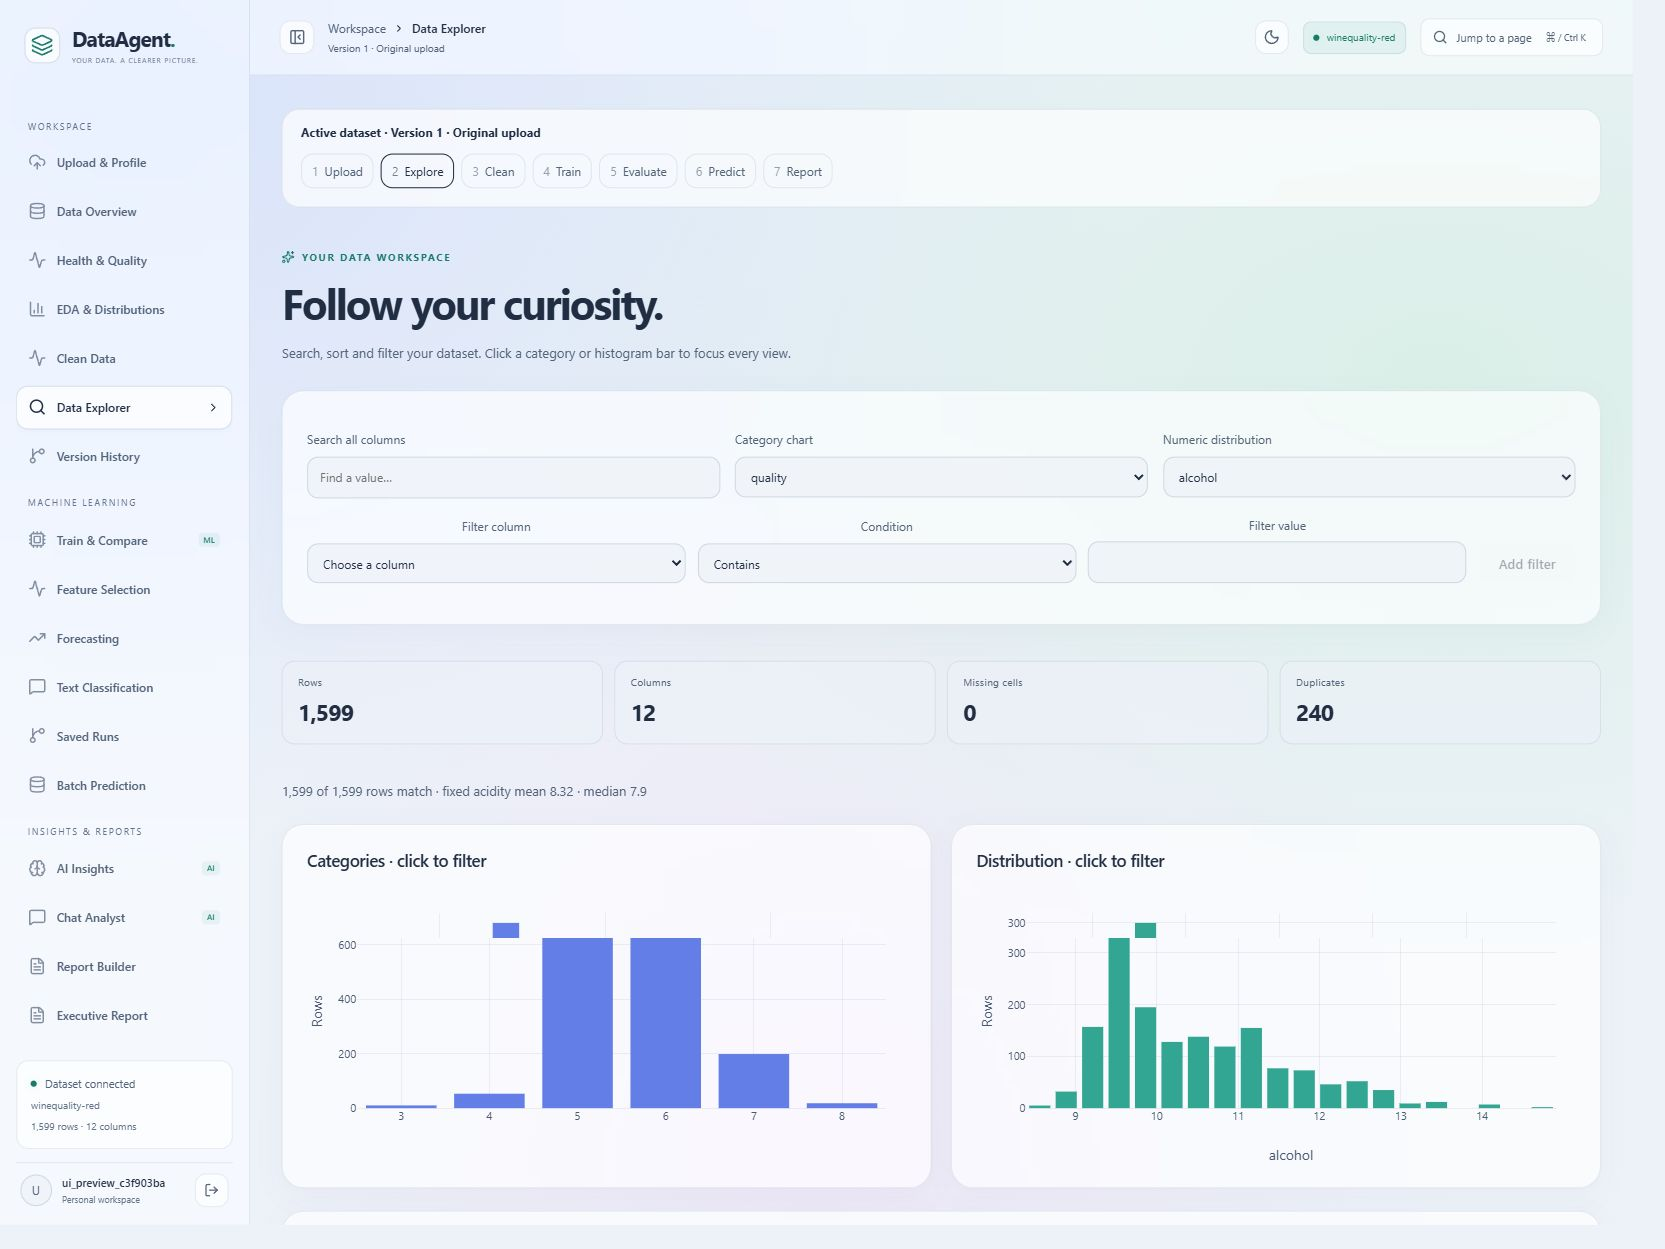
\includegraphics[width=\linewidth,height=9.2cm,keepaspectratio]{wine-explorer.jpg}
\par\vspace{3pt}\refstepcounter{figure}{\small\textbf{Figure \thefigure:} Wine explorer with quality categories, alcohol distribution and a sortable source table. Full distribution panels appear in the landscape plates.}
\end{center}

\subsection{Linked data exploration}
The explorer offers a searchable, sortable and paginated table with column filters. Category and histogram selections can apply related filters so that charts, counts and statistics refer to the same subset. The wine view selects quality categories and an alcohol distribution. Its unfiltered state retains all \textbf{1,599 rows}; a filtered subset must not be confused with full-dataset model evaluation.

\begin{center}\begin{tabular}{@{}lrrrr@{}}\toprule
\textbf{View} & \textbf{Rows} & \textbf{Columns} & \textbf{Missing cells} & \textbf{Duplicates}\\\midrule
Original wine dataset & 1,599 & 12 & 0 & 240\\
Deduplication preview & 1,359 & 12 & 0 & 0\\\bottomrule
\end{tabular}\end{center}

\subsection{Statistical interpretation}
The analytical services support checked statistical comparisons, effect sizes and corrections for multiple tests. Time-based interpretation requires suitable dates and aggregates; absent time information should produce an explicit limitation. Correlations and outlier flags are observations to investigate. An apparent extreme value may be valid, and a statistically significant relationship does not by itself imply practical importance or a causal mechanism.
\clearpage

% 12. AutoML
\section{Automated Machine Learning and Model Evaluation}
\subsection{Selection without holdout leakage}
The user selects a target, task and split strategy. Random splits suit independent observations; grouped splits keep entities separate; chronological splits reserve later observations. Group/date split columns are excluded from features. The application inspects candidate features and fits preprocessing and optional univariate selection within each validation fold~\cite{sklearn}.

For model $m$ with configuration $\theta$, selection follows
\[
(m^{*},\theta^{*})=\operatorname*{arg\,max}_{m,\theta}\;\frac{1}{K}\sum_{k=1}^{K}s\bigl(y_k,\widehat{f}^{(-k)}_{m,\theta}(X_k)\bigr),
\]
where $s$ is the validation score and preprocessing for fold $k$ is fitted without its validation rows. The selected candidate is evaluated on the separate holdout and compared with a simple training-derived baseline.

\reportfigure{\linewidth}{9.2cm}{wine-automl.jpg}{Wine-quality regression: selected Random Forest, holdout $R^2=0.5377$, validation leaderboard and saved artifact.}

\subsection{Models, tuning and explanations}
Candidate models include linear and regularised regressors, decision trees, random forests and optional boosted-tree libraries. Optuna tuning is retained only when validation supports the tuned candidate. Classification uses macro F1 as its primary score; regression reports R-squared and error measures. Confusion matrices, residual plots, feature importance and poor-holdout warnings support review.

Feature selection can compare all eligible and selected settings using the same estimator and folds. Probability reliability diagrams, Brier scores and threshold exploration are available for suitable classifiers~\cite{calibration}. Displayed probabilities remain labelled uncalibrated; threshold exploration on holdout data is exploratory rather than a fresh unbiased evaluation.
\clearpage

% 13. Specialised workflows
\section{Forecasting, Text Classification and Prediction}
\subsection{Forecasting on a regular calendar}
Users choose a date, outcome, calendar frequency, forecast horizon and optional series column. Missing periods either stop the run with an explanation or use explicitly selected past-only forward-fill. Earlier rolling windows select among simple forecasting candidates; later windows estimate interval widths; a final horizon measures untouched holdout error and observed coverage. Separate series are fitted independently.

The wine dataset has no suitable time index for this demonstration. Forecasting results elsewhere in this report use a separate passenger-series fixture; no wine forecast is implied.

\subsection{Text classification}
The text workflow fits TF-IDF features and compares Logistic Regression with Multinomial Naive Bayes. Normalized duplicate messages stay together across partitions. The interface reports per-class precision, recall and F1, a confusion matrix and misclassified holdout examples. The locally downloaded Kaggle copy of the SMS spam collection contains 5,572 messages; its recorded split achieved macro F1 0.9568 against a 0.4639 baseline~\cite{sms}.

\subsection{Saved models and batch inference}
Batch prediction validates a new CSV or Excel file against the saved artifact's schema. Missing columns and invalid numeric values are rejected; extra columns remain in the downloaded output. Missing feature values use the saved training preprocessing. Optional binary thresholds alter decisions without changing the model's probability estimates. Older-version artifacts require deliberate selection and retain their original schema.

Saved Runs preserves settings, version context, baselines and diagnostics for comparison. Matching metric names do not make runs with different targets, data versions or split strategies directly comparable.

\reportfigure{\linewidth}{8.2cm}{wine-report-builder.jpg}{Wine report builder with editable commentary, branding, selected evidence charts and a live preview.}
\clearpage

% 14. Results
\section{Experimental Results and Validation}
The recorded audit combines regression tests with interaction through the running React interface. Synthetic fixtures exercise known behaviours; real datasets exercise different formats and statistical structures. The values below describe specific runs and should not be interpreted as a general ranking of algorithms.

\begin{center}\small\begin{tabularx}{\linewidth}{@{}>{\raggedright\arraybackslash}p{4.7cm}>{\raggedright\arraybackslash}p{2.7cm}>{\raggedright\arraybackslash}X@{}}\toprule
\textbf{Experiment} & \textbf{Result} & \textbf{Evaluation context}\\\midrule
Red-wine quality regression & $R^2=0.5377$ & Saved random split: 1,279 train / 320 holdout\\
Synthetic regression, random & $R^2=0.9723$ & 192 training / 48 holdout records\\
Synthetic regression, grouped & $R^2=0.9876$ & Entity-separated holdout\\
Synthetic regression, chronological & $R^2=0.9860$ & Later-date holdout\\
Synthetic binary classification & Macro F1 = 1.0000 & Deliberately simple functional fixture\\
SMS spam classification & Macro F1 = 0.9568 & 4,457 training / 1,115 holdout messages\\
Two-series forecasting, North / South & MAE = 11.65 / 17.47 & Eight rolling windows; horizon six\\
Observed forecast interval coverage & 83.3\% & Final six-period holdout; low-coverage warning\\\bottomrule
\end{tabularx}\end{center}
\sourcehint{Recorded live audit dated 18 October 2026; project file \texttt{ML\_CLEANING\_TEST\_REPORT.md} and saved run diagnostics.}

\subsection{Functional and failure-path checks}
The full backend regression run passed \textbf{317 tests}; the frontend suite passed \textbf{21 tests}, and the production build completed. Coverage includes project ownership, stage error retention, constrained calculations, data fingerprints, cleaning protection, fold-safe model evaluation, state restoration and artifact downloads. Passing these tests establishes the checked software behaviour, not universal statistical or security correctness.

Live negative cases rejected missing batch columns and invalid numeric input. A forecast file with a missing month stopped until forward-fill was explicitly selected. An intentionally shifted chronological regression example displayed a poor-holdout warning. Cleaning previews preserved the original and provided reversible versions and detailed audit entries.

\subsection{Report generation and reproducibility}
The Report Builder allows users to select supported evidence charts, edit commentary and business context, set branding, save templates and export PDF or PowerPoint. Computed values and charts should be reviewed together before sharing. The present academic report was produced separately in LaTeX and includes screenshots of the application, rather than implying that its internal report exporter generated this document.

\subsection{Interpretation of the findings}
The wine run uses the original data, which contains exact duplicates; repeats across partitions can inflate evaluation. A deduplicated or duplicate-grouped rerun is needed before treating that score as robust evidence. Synthetic scores do not establish generalisation. Forecast intervals remain approximate. Independently labelled evaluation of LLM factuality, latency and cost remains future work.
\clearpage

% 15. Conclusion and references
\section{Conclusion and Future Scope}
Data Agent integrates Generative AI assistance with explicit data preparation, evaluated predictive models and reporting. The user can ask a question, inspect a computation, preview a transformation and trace a model result to a dataset version. The application demonstrates that conversational convenience can coexist with reproducible numerical services and visible limitations.

The current implementation provides specialised analytical stages, guided cleaning, exploratory views, supervised AutoML, forecasting, text classification, saved runs and validated prediction. Its main engineering lessons are to retain dependency and error information, fit learned transformations within evaluation boundaries, reject invalid inputs and preserve provenance when data changes.

Future work should prioritise a labelled benchmark for generated explanations, validation-set threshold selection and probability calibration, wider forecasting backtests, stronger deployment isolation, and measurements of latency and cost. Larger-scale workers and additional modeling tasks can follow once these evaluation and deployment foundations are measured. Human review remains necessary for sensitive or consequential use.

\vspace{.15cm}
\begingroup
\small
\renewcommand{\refname}{References}
\addcontentsline{toc}{section}{References}
\begin{thebibliography}{9}
\raggedright
\setlength{\itemsep}{2pt}
\bibitem{react} S. Yao et al., ``ReAct: Synergizing Reasoning and Acting in Language Models,'' ICLR, 2023. \url{https://arxiv.org/abs/2210.03629}.
\bibitem{autogen} Q. Wu et al., ``AutoGen: Enabling Next-Gen LLM Applications via Multi-Agent Conversation,'' arXiv:2308.08155, 2023. \url{https://arxiv.org/abs/2308.08155}.
\bibitem{sklearn} Scikit-learn developers, ``Common pitfalls and recommended practices,'' documentation. \url{https://scikit-learn.org/stable/common_pitfalls.html}. Accessed 18 October 2026.
\bibitem{optuna} T. Akiba, S. Sano, T. Yanase, T. Ohta and M. Koyama, ``Optuna: A Next-generation Hyperparameter Optimization Framework,'' KDD, 2019. \url{https://arxiv.org/abs/1907.10902}.
\bibitem{calibration} Scikit-learn developers, ``Probability calibration,'' documentation. \url{https://scikit-learn.org/stable/modules/calibration.html}. Accessed 18 October 2026.
\bibitem{sms} UCI Machine Learning Repository, ``SMS Spam Collection,'' public dataset; project copy downloaded through Kaggle. \url{https://archive.ics.uci.edu/dataset/228/sms+spam+collection}.
\bibitem{implementation} B. L. R. Palem, \textit{Data Agent project implementation and verification records}, local repository, October 2026. Relevant modules: \texttt{backend/graph/workflow.py}, \texttt{backend/services/automl\_engine.py}, workspace services and React pages; recorded audit: \texttt{ML\_CLEANING\_TEST\_REPORT.md}.
\end{thebibliography}
\endgroup

\clearpage
\newgeometry{left=1.2cm,right=1.2cm,top=1.25cm,bottom=1.25cm,headheight=15pt,headsep=10pt}
\begin{landscape}
\pdfpageattr{/Rotate 90}
\section*{Desktop Application Plates}
\thispagestyle{empty}
\addcontentsline{toc}{section}{Desktop Application Plates}
\noindent\textbf{Plate A: Wine-quality overview.} Original upload: 1,599 records, 12 columns, 240 exact duplicates. The dashboard's 66/100 quality score is a heuristic.
\begin{center}
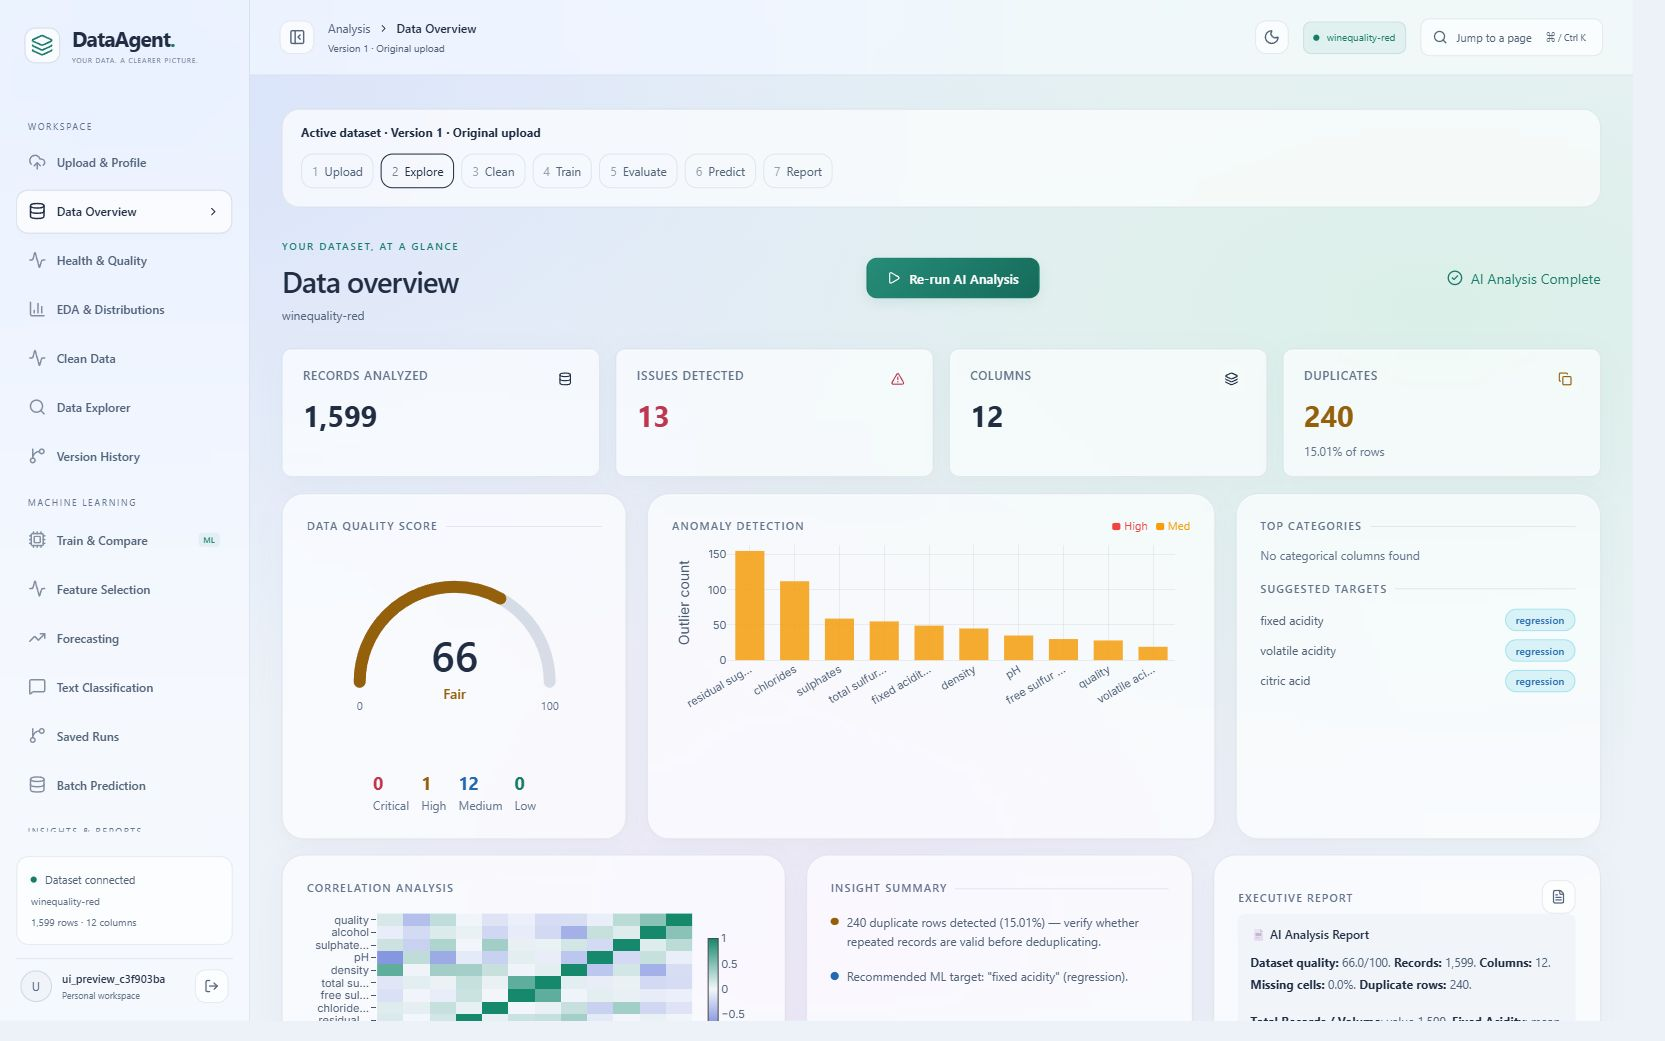
\includegraphics[width=\linewidth,height=15.7cm,keepaspectratio]{wine-overview.jpg}
\end{center}
\noindent\hfill{\small\thepage}\hfill\null
\clearpage
\section*{Desktop Application Plates -- Distributions}
\thispagestyle{empty}
\noindent\textbf{Plate B: Wine-quality EDA.} Desktop distribution panels show all 12 columns, with descriptive summaries and chart axes. These patterns are exploratory.
\begin{center}
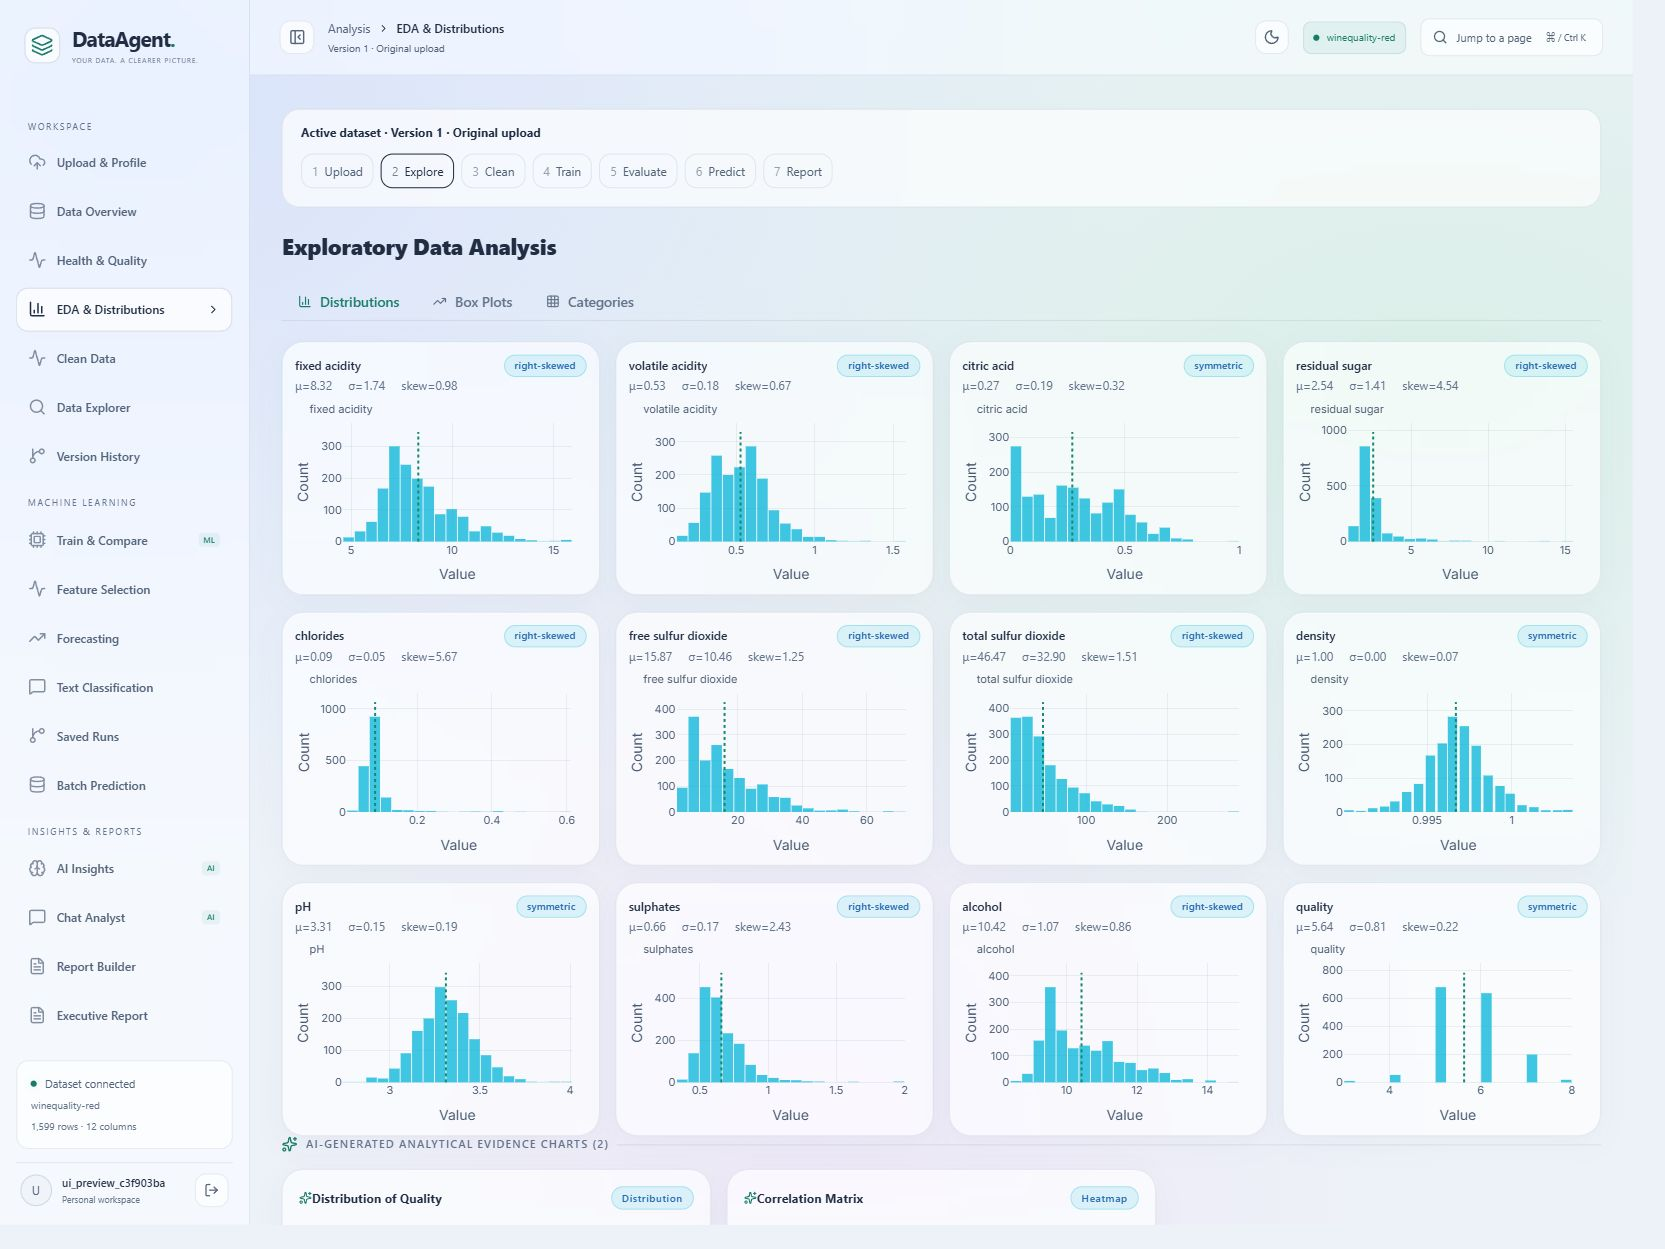
\includegraphics[width=\linewidth,height=15.7cm,keepaspectratio]{wine-eda.jpg}
\end{center}
\noindent\hfill{\small\thepage}\hfill\null
\end{landscape}
\pdfpageattr{/Rotate 0}
\restoregeometry
\end{document}
